% Drawing 138/06-49 -- folder 138, batch 06, archive page 118 (PDF page 119).
% Transcription: une esquisse biffée ($\mathbb{Z}$) ; deux cercles reliés par un segment, $\mathbb{Z}_2 \times \mathbb{Z}_2$ ; un cercle avec une queue terminée par une fourche, $\mathbb{Z}_2$ ; deux fourches reliées par un segment, $\mathbb{Z}_2 \times \mathbb{Z}_2$. En bas de page : une ellipse partagée par un diamètre, $\mathbb{Z}_2 \cdot \mathfrak{S}_3$ ; une esquisse biffée ; deux ellipses traversées d'arêtes, $\mathbb{Z}_2 \times \mathbb{Z}_2$ et $\mathbb{Z}_2 \times \mathbb{Z}_2$.
% Kind: table of small maps with automorphism groups (degree 6, e). Method 2 (schematic redraw from the facsimile). Status: partial.
% Notes: e): a struck sketch (heavily scribbled, grey outline only; « Z » under it); two circles joined by a segment, Z_2 x Z_2; a circle with a tail ending in a fork, Z_2; two forks joined by a segment, Z_2 x Z_2. At the bottom of the page: an ellipse divided by a diameter, Z_2 . S_3; a struck sketch; two ellipses crossed by edges, Z_2 x Z_2 and Z_2 x Z_2 (the bottom row touches the page edge). Each small map carries its automorphism group as written (given as labels, since the transcription names them); vertex positions and loop shapes approximate.
% Coordinates: 1 unit = 1 mm = 1/100 of the crop width (bbox in page fractions: [0.198, 0.715, 0.886, 0.881]).
% Redrawn by Claude (claude-opus-5-5), issue #73, 2026-11-07; not checked by a human; not compiled (no TeX in the session).
% Rights: reproduces part of the work -- behind RENDER_TRANSCRIPTS, never published by itself.
\documentclass[tikz,border=3pt]{standalone}
\usepackage{amsmath,amssymb}
\usetikzlibrary{patterns,arrows.meta}
\tikzset{pencil/.style={black!45}, struck/.style={black!35}, mark/.style={circle,draw,inner sep=1.3pt}, pt/.style={circle,fill,inner sep=0.9pt}, opt/.style={circle,draw,fill=white,inner sep=1.1pt}}
\begin{document}
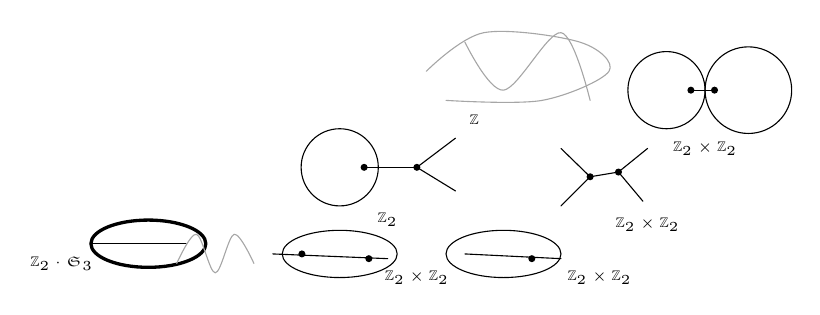
\begin{tikzpicture}[x=1mm,y=1mm,line cap=round,line join=round,font=\scriptsize]
\draw[struck] plot[smooth, tension=0.55] coordinates {(51.2,-6.1) (58.5,-1.2) (70.7,-2.4) (74.4,-6.1) (65.9,-9.8) (53.7,-9.8)};
\draw[struck] plot[smooth, tension=0.55] coordinates {(56.1,-2.4) (61,-8.5) (68.3,-1.2) (72,-9.8)};
\node[inner sep=1pt] at (57.3,-12.2) {\tiny $\mathbb{Z}$};
\draw (81.7,-8.5) circle[radius=4.9];
\draw (92.1,-8.5) circle[radius=5.5];
\draw (84.8,-8.5) -- (87.8,-8.5);
\node[pt] at (84.8,-8.5) {};
\node[pt] at (87.8,-8.5) {};
\node[inner sep=1pt] at (86.6,-15.9) {\tiny $\mathbb{Z}_2\times\mathbb{Z}_2$};
\draw (40.2,-18.3) circle[radius=4.9];
\draw (43.3,-18.3) -- (50,-18.3);
\draw (50,-18.3) -- (54.9,-14.6);
\draw (50,-18.3) -- (54.9,-21.3);
\node[pt] at (43.3,-18.3) {};
\node[pt] at (50,-18.3) {};
\node[inner sep=1pt] at (46.3,-25) {\tiny $\mathbb{Z}_2$};
\draw (72,-19.5) -- (75.6,-18.9);
\draw (72,-19.5) -- (68.3,-15.9);
\draw (72,-19.5) -- (68.3,-23.2);
\draw (75.6,-18.9) -- (79.3,-15.9);
\draw (75.6,-18.9) -- (78.7,-22.6);
\node[pt] at (72,-19.5) {};
\node[pt] at (75.6,-18.9) {};
\node[inner sep=1pt] at (79.3,-25.6) {\tiny $\mathbb{Z}_2\times\mathbb{Z}_2$};
\draw[very thick] (15.9,-28) ellipse[x radius=7.3, y radius=3];
\draw (8.5,-28) -- (20.7,-28);
\node[inner sep=1pt] at (4.9,-30.5) {\tiny $\mathbb{Z}_2\cdot\mathfrak{S}_3$};
\draw[struck] plot[smooth, tension=0.55] coordinates {(19.5,-30.5) (22,-26.8) (24.4,-31.7) (26.8,-26.8) (29.3,-30.5)};
\draw (40.2,-29.3) ellipse[x radius=7.3, y radius=3];
\draw (31.7,-29.3) -- (46.3,-29.9);
\node[pt] at (35.4,-29.3) {};
\node[pt] at (43.9,-29.9) {};
\node[inner sep=1pt] at (50,-32.3) {\tiny $\mathbb{Z}_2\times\mathbb{Z}_2$};
\draw (61,-29.3) ellipse[x radius=7.3, y radius=3];
\draw (56.1,-29.3) -- (68.3,-29.9);
\node[pt] at (64.6,-29.9) {};
\node[inner sep=1pt] at (73.2,-32.3) {\tiny $\mathbb{Z}_2\times\mathbb{Z}_2$};
\end{tikzpicture}
\end{document}
